%% =====================================================================
%% Slide thuyết trình — Data Engineering (CO5173), HCMUT — Nhóm 27
%% Kho dữ liệu Kimball cho phân tích dòng tiền ngân hàng (dữ liệu Berka)
%%
%% Nội dung lấy từ report/main.tex. Ảnh chụp ứng dụng: report/figures/.
%% Biên dịch bằng XeLaTeX:  tectonic slides.tex   (Overleaf: chọn compiler XeLaTeX)
%% =====================================================================
\documentclass[aspectratio=169,11pt]{beamer}

\usepackage{fontspec}
% TeX Gyre fonts by file name (cover Vietnamese; work in tectonic and on Overleaf)
\setsansfont{texgyreheros}[Extension=.otf, UprightFont=*-regular, BoldFont=*-bold,
  ItalicFont=*-italic, BoldItalicFont=*-bolditalic]
\setmonofont{texgyrecursor}[Extension=.otf, UprightFont=*-regular, BoldFont=*-bold,
  ItalicFont=*-italic, BoldItalicFont=*-bolditalic]
\usepackage{booktabs}
\usepackage{amssymb}
\usepackage{array}
\usepackage{graphicx}
\usepackage{tikz}
\usetikzlibrary{arrows.meta,positioning,fit,calc}
\usepackage{pgfplots}
\pgfplotsset{compat=1.18}
\graphicspath{{../report/figures/}}

% ---------- Theme ----------
\definecolor{navy}{HTML}{1F3A5F}
\definecolor{accent}{HTML}{C0392B}
\definecolor{chcol}{HTML}{E0A100}
\definecolor{pgcol}{HTML}{336791}
\definecolor{obtcol}{HTML}{8E7CC3}
\definecolor{okcol}{HTML}{2E7D32}
\definecolor{soft}{HTML}{F3F5F8}
\usetheme{default}
\setbeamercolor{frametitle}{fg=navy}
\setbeamercolor{title}{fg=navy}
\setbeamercolor{structure}{fg=navy}
\setbeamercolor{itemize item}{fg=accent}
\setbeamercolor{itemize subitem}{fg=navy}
\setbeamercolor{block title}{bg=navy,fg=white}
\setbeamercolor{block body}{bg=soft}
\setbeamerfont{frametitle}{size=\Large,series=\bfseries}
\setbeamertemplate{navigation symbols}{}
\setbeamertemplate{itemize items}[circle]
\setbeamertemplate{blocks}[rounded][shadow=false]
\setbeamertemplate{footline}{%
  \hbox{\begin{beamercolorbox}[wd=\paperwidth,ht=3ex,dp=1.2ex]{}%
    \hspace{1.2em}{\tiny\color{gray}Nhóm 27 · CO5173 Data Engineering · Kho dữ liệu Kimball cho dòng tiền ngân hàng}%
    \hfill{\tiny\color{gray}\insertsection\quad\insertframenumber/\inserttotalframenumber}\hspace{1.2em}%
  \end{beamercolorbox}}}
\AtBeginSection[]{%
  \begin{frame}[plain]
    \vfill
    {\color{gray}\small Phần \thesection}\par\medskip
    {\color{navy}\Huge\bfseries\insertsectionhead}\par\bigskip
    {\color{accent}\rule{6em}{2pt}}
    \vfill
  \end{frame}}

\newcommand{\tbl}[1]{\texttt{#1}}
% TikZ styles with a parameter must be defined outside frames (beamer reads frames as arguments)
\tikzset{
  box/.style={draw, rounded corners=3pt, align=center, minimum height=1.05cm, text width=2.5cm,
              font=\footnotesize, fill=#1},
  box/.default=white,
  ent/.style={draw, rounded corners=2pt, font=\scriptsize, align=center, inner sep=3pt, fill=#1},
  ent/.default=green!10}
\newcolumntype{L}[1]{>{\raggedright\arraybackslash}p{#1}}
\newcommand{\good}{{\color{okcol}$\checkmark$}}
\newcommand{\bad}{{\color{accent}$\times$}}

\title{Kho dữ liệu Kimball cho phân tích dòng tiền ngân hàng}
\subtitle{Thiết kế, triển khai và đánh giá với Spark, ClickHouse và PostgreSQL}
\author{Kiet Ho Tuan Nguyen \and Quan Minh Tran \and Van Ngoc Huynh \and Hai Ngoc Ho}
\institute{Nhóm 27 · Data Engineering (CO5173) · HK1 2026--2027\\
Trường Đại học Bách khoa -- ĐHQG TP.HCM\\
GVHD: Assoc. Prof. Dr. Chau Thi Ngoc Vo}
\date{}

\begin{document}

\begin{frame}[plain]
  \titlepage
\end{frame}

\begin{frame}{Nội dung}
  \tableofcontents
\end{frame}

%% =====================================================================
\section{Bài toán}

\begin{frame}{Bối cảnh: ngân hàng cần ba loại câu trả lời đáng tin}
  \begin{columns}[T]
    \column{0.55\textwidth}
    \begin{itemize}
      \item \textbf{Dòng tiền:} tiền vào, tiền ra, dòng tiền thuần theo kỳ và theo hạng khách hàng
      \item \textbf{Từng tài khoản:} lịch sử giao dịch, dấu hiệu gian lận, kết quả xử lý
      \item \textbf{Độ tin cậy:} lần nạp có thành công không, bản ghi nào bị loại, báo cáo cũ có bị thay đổi không
    \end{itemize}
    \column{0.42\textwidth}
    \begin{block}{Câu hỏi nghiên cứu}
      \small Làm thế nào biến dữ liệu giao dịch ngân hàng thành một kho dữ liệu \textbf{đúng}, \textbf{nhanh}, \textbf{khai thác được}, có kiểm soát việc nạp và \textbf{giữ được lịch sử}?
    \end{block}
  \end{columns}
  \bigskip
  \small Giải pháp: \textbf{kho dữ liệu Kimball} trên ClickHouse, pipeline theo lô bằng Spark, kho vận hành PostgreSQL, ứng dụng Streamlit 3 tab.
\end{frame}

\begin{frame}{3 nhóm người dùng, 8 yêu cầu nghiệp vụ}
  \footnotesize
  \begin{tabular}{L{2.3cm} L{1.4cm} L{8.9cm}}
    \toprule
    \textbf{Người dùng} & \textbf{Tab} & \textbf{Yêu cầu nghiệp vụ (BR)} \\
    \midrule
    U01 Quản lý kinh doanh & Tổng quan & BR01 tổng quan dòng tiền: vào, ra, thuần, số giao dịch, theo hạng, biểu đồ ngày/tháng \\
    \midrule
    U02 Chuyên viên phân tích & Phân tích & BR02 tra cứu hoạt động một tài khoản \newline
      BR03 phát hiện gian lận, cảnh báo kèm lý do và căn cứ \newline
      BR04 theo dõi xử lý cảnh báo: chưa xem → đang xem xét → đã xử lý, ghi chú \\
    \midrule
    U03 Kỹ sư dữ liệu & Vận hành & BR05 kiểm soát dữ liệu, tách bản ghi lỗi \newline
      BR06 giám sát pipeline: bước, trạng thái, thời gian, nguyên nhân lỗi \newline
      BR07 sao lưu, khôi phục 6 bảng của kho \newline
      BR08 báo cáo lịch sử: đổi hạng không làm thay đổi báo cáo kỳ cũ (SCD2) \\
    \bottomrule
  \end{tabular}
  \medskip

  \small Mỗi BR có một \textbf{kịch bản đánh giá} (KB01--KB08) với kết quả mong đợi viết \emph{trước} khi nạp.
\end{frame}

\begin{frame}{Nguồn dữ liệu: Berka (ngân hàng Séc, PKDD'99)}
  \begin{columns}[T]
    \column{0.48\textwidth}
    \small
    \begin{itemize}
      \item \textbf{1.056.320} giao dịch, \textbf{4.500} tài khoản, 5.369 khách, 77 khu vực, 1993--1998
      \item Mỗi tài khoản đúng \textbf{1 chủ sở hữu} (OWNER); 409 tài khoản mở ở khu vực khác nơi ở của chủ
      \item Giao dịch tăng hằng năm: 28.205 (1993) → 322.277 (1998)
      \item Số tiền không âm; chiều tiền suy ra từ mã loại giao dịch
    \end{itemize}
    \column{0.5\textwidth}
    \footnotesize
    \setlength{\tabcolsep}{3pt}
    \begin{tabular}{l c r r}
      \toprule
      \textbf{Loại} & \textbf{Chiều} & \textbf{Số GD} & \textbf{Tổng (tr. CZK)} \\
      \midrule
      VYDAJ (chi) & ra & 634.571 & 2.821,7 \\
      PRIJEM (thu) & vào & 405.083 & 3.227,5 \\
      VYBER (rút) & ra & 16.666 & 208,6 \\
      \bottomrule
    \end{tabular}
    \medskip

    \textbf{Hạng thành viên mô phỏng} (Berka không có):\\
    theo tiền vào năm đầu → Standard 2.075 · Silver 1.438 · Gold 698 · Platinum 289.
    Đánh giá lại cuối 1998 → \textbf{618 khách đổi hạng} từ 01/01/1999.
  \end{columns}
\end{frame}

\begin{frame}{Lỗi dữ liệu nguồn (theo ISO/IEC 25012)}
  \footnotesize
  \begin{tabular}{L{1.9cm} L{6.2cm} L{4.6cm}}
    \toprule
    \textbf{Đặc tính} & \textbf{Phát hiện} & \textbf{Cách xử lý} \\
    \midrule
    Đầy đủ & \tbl{operation} trống ở 183.114 giao dịch; \tbl{k\_symbol} NULL 481.881 + chuỗi trắng 53.433 & Gán \tbl{NOT\_RECORDED}, không bỏ dòng nào \\
    Nhất quán & Hai cách ghi ``thiếu''; mã có khoảng trắng; 17 tổ hợp mã thực chất là 15 & Chuẩn hóa → 15 tổ hợp (junk dimension) \\
    Dễ hiểu & Mã tiếng Séc (PRIJEM, VYDAJ, SIPO…) & Tên dễ đọc + chiều tiền vào/ra \\
    Chính xác & Ngày sinh và giới tính gộp trong ``birth number'' & Tách thành \tbl{gender}, \tbl{birth\_date} \\
    Cập nhật & Không có thuộc tính nào có lịch sử thay đổi & Hạng thành viên mô phỏng có ngày hiệu lực \\
    \bottomrule
  \end{tabular}
\end{frame}

%% =====================================================================
\section{Giải pháp đề xuất}

\begin{frame}{Kiến trúc A--F}
  \centering
  \resizebox{\textwidth}{!}{%
  \begin{tikzpicture}[
    arr/.style={-{Stealth[length=2mm]}, thick}, lbl/.style={font=\scriptsize, above=1pt}]
    \node[box=gray!12] (src) at (0,0) {\textbf{A. Nguồn}\\{\scriptsize Berka, hạng, file kịch bản}};
    \node[box=gray!12, minimum height=0.8cm] (lake) at (3.7,2.0) {\textbf{B. Data Lake}\\{\scriptsize Parquet theo lô}};
    \node[box=blue!10, minimum height=1.5cm] (pipe) at (3.7,0) {\textbf{C. Pipeline}\\{\scriptsize PySpark: kiểm tra, chuẩn hóa, SCD2, nạp, đối chiếu, cảnh báo}};
    \node[box=yellow!25] (dw) at (8.1,1.3) {\textbf{D. ClickHouse}\\{\scriptsize star schema + vùng sao lưu}};
    \node[box=blue!15] (ops) at (8.1,-1.3) {\textbf{E. PostgreSQL}\\{\scriptsize lần chạy, lỗi, cảnh báo, xử lý}};
    \node[box=red!10, minimum height=2.2cm] (app) at (12.4,0) {\textbf{F. Ứng dụng}\\Streamlit\\{\scriptsize Tổng quan · Phân tích · Vận hành}};
    \draw[arr] (src) -- node[lbl]{lô} (pipe);
    \draw[arr, dashed] (pipe.north) -- node[right, font=\scriptsize]{chụp đầu vào} (lake.south);
    \draw[arr] ([yshift=3mm]pipe.east) -- node[lbl, sloped]{nạp} (dw.west);
    \draw[arr] ([yshift=-3mm]pipe.east) -- node[lbl, sloped]{ghi log} (ops.west);
    \draw[arr] (dw.east) -- node[lbl, sloped]{đọc} ([yshift=5mm]app.west);
    \draw[arr, <->] (ops.east) -- node[lbl, sloped]{xử lý} ([yshift=-5mm]app.west);
    \draw[arr, dashed] (app.south) -- ++(0,-1.6) -| node[pos=0.25, above, font=\scriptsize]{lệnh: chạy, chạy lại, sao lưu, khôi phục} (pipe.south);
  \end{tikzpicture}}
  \medskip

  \small Tách rõ \textbf{lưu trữ} (B, D, E), \textbf{xử lý} (C) và \textbf{ứng dụng} (F). Xử lý theo lô: 1 lô tham chiếu + 72 lô tháng + 4 lô kịch bản.
\end{frame}

\begin{frame}{Mô hình dữ liệu Kimball}
  \begin{columns}[c]
    \column{0.47\textwidth}
    \centering
    \resizebox{\linewidth}{!}{%
    \begin{tikzpicture}
      \node[ent=blue!12, text width=3.0cm] (f) at (0,0) {\textbf{fact\_transaction}\\1 dòng / giao dịch\\\texttt{amount}, \texttt{balance\_after}};
      \node[ent] (d) at (-2.7,1.8) {dim\_date};
      \node[ent] (c) at (2.7,1.8) {dim\_customer\\\textbf{SCD Type 2}};
      \node[ent] (a) at (-2.7,-1.8) {dim\_account};
      \node[ent] (t) at (2.7,-1.8) {dim\_transaction\_profile\\(junk)};
      \node[ent=orange!15] (g) at (0,-3.3) {dim\_district};
      \draw (f)--(d); \draw (f)--(c); \draw (f)--(a); \draw (f)--(t);
      \draw[dashed] (a.south) |- node[pos=0.75, below, font=\tiny]{chi nhánh} (g.west);
      \draw[dashed] (c.east) -- ++(0.5,0) |- node[pos=0.75, below, font=\tiny]{nơi ở} (g.east);
    \end{tikzpicture}}
    \column{0.5\textwidth}
    \small
    \begin{itemize}
      \item \textbf{Grain:} 1 dòng / giao dịch → trả lời được cả báo cáo lẫn tra cứu chi tiết
      \item \textbf{amount} cộng được; \textbf{balance\_after} không cộng qua thời gian
      \item \textbf{dim\_customer} SCD2: mỗi hạng một phiên bản, khóa thay thế riêng, \tbl{valid\_from}–\tbl{valid\_to}
      \item \textbf{dim\_district} đóng 2 vai trò: chi nhánh và nơi ở
      \item \textbf{Junk dimension}: 15 tổ hợp loại / phương thức / mục đích + chiều tiền
    \end{itemize}
  \end{columns}
\end{frame}

\begin{frame}{Ví dụ SCD Type 2: khách 24 đổi hạng}
  \begin{columns}[T]
    \column{0.52\textwidth}
    \footnotesize
    \tbl{dim\_customer} của khách 24:\par\smallskip
    \scriptsize\setlength{\tabcolsep}{3pt}
    \begin{tabular}{r l l l c}
      \toprule
      \textbf{sk} & \textbf{Hạng} & \textbf{Từ} & \textbf{Đến} & \textbf{Hiện tại} \\
      \midrule
      18 & Standard & 1993-05-26 & 1999-01-01 & 0 \\
      4.501 & Silver & 1999-01-01 & 2299-12-31 & 1 \\
      \bottomrule
    \end{tabular}
    \bigskip

    \small Mỗi giao dịch nối tới phiên bản \textbf{có hiệu lực tại ngày giao dịch}:
    \begin{itemize}
      \item giao dịch 1993--1998 → sk 18 (Standard)
      \item giao dịch từ 01/01/1999 → sk 4.501 (Silver)
    \end{itemize}
    \column{0.45\textwidth}
    \begin{block}{Vì sao quan trọng (BR08)}
      \small Đổi hạng 618 khách \textbf{không sửa} dòng fact nào của kỳ cũ.\\[3pt]
      → Báo cáo 1993--1998 theo hạng \textbf{giữ nguyên} sau khi nạp KB08.\\[3pt]
      → Kỳ mới (01/1999) tính theo hạng mới.
    \end{block}
    \smallskip
    \footnotesize Điều kiện ngày nằm \emph{trong} phép join: giao dịch không có phiên bản hợp lệ bị tách theo quy tắc V7 thay vì âm thầm biến mất.
  \end{columns}
\end{frame}

\begin{frame}{Pipeline theo lô: kiểm soát từng lô}
  \centering
  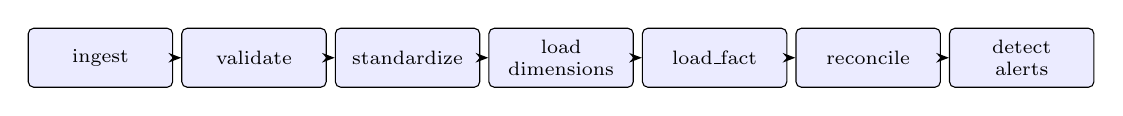
\begin{tikzpicture}[st/.style={draw, rounded corners=2pt, fill=blue!8, font=\scriptsize, minimum height=0.75cm, text width=1.6cm, align=center}, arr/.style={-{Stealth[length=1.6mm]}, thick}]
    \node[st] (in) at (1.95,0) {ingest};
    \node[st] (va) at (3.90,0) {validate};
    \node[st] (st) at (5.85,0) {standardize};
    \node[st] (di) at (7.80,0) {load\\dimensions};
    \node[st] (fa) at (9.75,0) {load\_fact};
    \node[st] (re) at (11.70,0) {reconcile};
    \node[st] (al) at (13.65,0) {detect\\alerts};
    \draw[arr] (in) -- (va); \draw[arr] (va) -- (st); \draw[arr] (st) -- (di);
    \draw[arr] (di) -- (fa); \draw[arr] (fa) -- (re); \draw[arr] (re) -- (al);
  \end{tikzpicture}
  \medskip

  \begin{columns}[T]
    \column{0.5\textwidth}
    \footnotesize
    \textbf{7 quy tắc chất lượng (BR05):}\\
    V1 thiếu trường bắt buộc · V2 tài khoản không tồn tại · V3 số tiền âm / không phải số · V4 ngày sai · V5 mã loại lạ · V6 trùng mã giao dịch · V7 không có phiên bản chủ sở hữu hợp lệ\\[4pt]
    Bản ghi lỗi \textbf{bị tách} kèm quy tắc, lý do, nội dung gốc; phần còn lại của lô vẫn được nạp.
    \column{0.46\textwidth}
    \footnotesize
    \textbf{Mỗi lần chạy được ghi lại (BR06):} bước, trạng thái, thời gian, số nhận / đạt / lỗi, nguyên nhân thất bại.\\[4pt]
    \textbf{Chạy lại không trùng:} bỏ qua giao dịch lô đã nạp; bảng fact là ReplacingMergeTree theo mã giao dịch.\\[4pt]
    \textbf{Đối chiếu từng lô:} số dòng và tiền vào/ra của kho = đầu vào.
  \end{columns}
\end{frame}

\begin{frame}{Cảnh báo gian lận (BR03) và xử lý (BR04)}
  \begin{columns}[T]
    \column{0.5\textwidth}
    \small
    \textbf{Quy tắc dễ giải thích}, tham số lưu trong \tbl{ops.alert\_rule}:
    \begin{itemize}
      \item \textbf{R1} tiền ra tăng mạnh: tiền ra trong tháng > 3 lần trung bình 6 tháng trước và > 50.000 CZK
      \item \textbf{R2} tài khoản ngủ đông: không giao dịch ≥ 180 ngày rồi có giao dịch ra
    \end{itemize}
    Duy nhất theo (tài khoản, quy tắc, kỳ) → chạy lại không sinh cảnh báo trùng.
    \column{0.47\textwidth}
    \begin{block}{Ví dụ: tài khoản 11, tháng 02/1999}
      \small Tiền ra \textbf{60.000 CZK}, gấp \textbf{19,5 lần} trung bình 6 tháng trước (3.075 CZK) → cảnh báo R1 kèm căn cứ và giao dịch liên quan.
    \end{block}
    \medskip
    \centering
    \begin{tikzpicture}[s/.style={draw, rounded corners=2pt, font=\scriptsize, fill=soft, minimum width=1.7cm, minimum height=0.6cm}, arr/.style={-{Stealth[length=1.6mm]}, thick}]
      \node[s] (n) at (0,0) {chưa xem};
      \node[s] (r) at (2.3,0) {đang xem xét};
      \node[s] (d) at (4.6,0) {đã xử lý};
      \draw[arr] (n) -- (r); \draw[arr] (r) -- (d);
      \draw[arr] (n.south) to[bend right=25] (d.south);
      \draw[arr, dashed] (d.north) to[bend right=25] node[above, font=\tiny]{mở lại} (r.north);
    \end{tikzpicture}\\
    \footnotesize Mỗi lần đổi trạng thái kèm ghi chú, người xử lý, thời điểm.
  \end{columns}
\end{frame}

\begin{frame}{Kho vận hành PostgreSQL và sao lưu (BR07)}
  \begin{columns}[T]
    \column{0.52\textwidth}
    \small
    \textbf{Kho vận hành (schema \tbl{ops})} lưu những gì phải \textbf{sửa tại chỗ và kiểm toán được}:
    \begin{itemize}
      \item lô, lần chạy, bước; bản ghi bị tách
      \item quy tắc và cảnh báo; lịch sử xử lý
      \item danh mục và kết quả sao lưu / khôi phục
    \end{itemize}
    Có khóa chính, khóa ngoại, CHECK, và hàm chỉ cho phép chuyển trạng thái hợp lệ.
    \column{0.45\textwidth}
    \small
    \textbf{Sao lưu / khôi phục} 6 bảng của kho (cả lịch sử SCD) bằng \tbl{BACKUP} / \tbl{RESTORE} của ClickHouse vào vùng lưu riêng.\\[4pt]
    Sau khôi phục, đối chiếu \textbf{5 nhóm số liệu}: số dòng, tiền vào, tiền ra, báo cáo theo hạng, phiên bản SCD.\\[4pt]
    \footnotesize Ghi chú của chuyên viên không trộn với số liệu ngân hàng; khôi phục kho không làm mất nhật ký vận hành.
  \end{columns}
\end{frame}

\begin{frame}{Ứng dụng: 3 tab cho 3 nhóm người dùng}
  \footnotesize
  \begin{tabular}{L{1.7cm} L{2.1cm} L{8.8cm}}
    \toprule
    \textbf{Tab} & \textbf{BR} & \textbf{Hiển thị và thao tác} \\
    \midrule
    Tổng quan & BR01 & Chọn kỳ; thẻ KPI; biểu đồ tiền vào / ra theo ngày hoặc tháng; bảng theo hạng \\
    Phân tích & BR02, BR03, BR04 & Tra cứu tài khoản; danh sách cảnh báo, lý do, căn cứ, giao dịch liên quan; form đổi trạng thái + ghi chú \\
    Vận hành & BR05--BR08 & Lần chạy và bước; bản ghi bị tách; sao lưu / khôi phục; báo cáo theo hạng kỳ cũ / kỳ mới \\
    Vận hành & Kịch bản & Chọn kịch bản → \textbf{xem trước} (chưa ghi gì) → chạy → so mong đợi với thực tế → chạy lại \\
    \bottomrule
  \end{tabular}
  \bigskip

  \small Ứng dụng không chỉ đọc mà còn \textbf{điều khiển}: lệnh chạy, chạy lại, sao lưu, khôi phục đi qua một dịch vụ \emph{runner} chỉ chấp nhận danh sách lệnh cho phép, mỗi lúc một việc; lần chạy được ghi là \tbl{triggered\_by = app}.
\end{frame}

\begin{frame}{Công nghệ và lý do chọn}
  \footnotesize
  \begin{tabular}{L{2.2cm} L{3.2cm} L{7.2cm}}
    \toprule
    \textbf{Khối} & \textbf{Công nghệ} & \textbf{Lý do} \\
    \midrule
    B. Data Lake & Parquet theo lô & Giữ nguyên đầu vào để truy vết và chạy lại \\
    C. Pipeline & Apache Spark (PySpark) & Quy tắc kiểm tra viết khai báo; cùng code chạy được trên cluster \\
    D. Kho dữ liệu & ClickHouse & Lưu theo cột, nén tốt, tổng hợp nhanh; BACKUP / RESTORE sẵn có \\
    E. Kho vận hành & PostgreSQL & Ràng buộc, transaction, sửa tại chỗ \\
    F. Ứng dụng & Streamlit & Cần \textbf{ghi} (xử lý cảnh báo) và \textbf{điều khiển} pipeline, không chỉ vẽ biểu đồ \\
    Triển khai & Docker Compose & Chạy lại được trên một máy \\
    \bottomrule
  \end{tabular}
  \bigskip

  \small Điểm yếu của ClickHouse với Kimball (không UPDATE tại chỗ, không ép khóa) được xử lý bằng: dimension dạng ReplacingMergeTree (ghi phiên bản mới, đọc bằng FINAL), pipeline tự cấp và kiểm tra khóa.
\end{frame}

%% =====================================================================
\section{Phương án thay thế và cách đánh giá}

\begin{frame}{Các phương án so sánh: mỗi phép chỉ đổi một yếu tố}
  \footnotesize
  \begin{tabular}{l L{3.4cm} L{2.3cm} L{5.8cm}}
    \toprule
    \textbf{Mã} & \textbf{So sánh} & \textbf{Giữ nguyên} & \textbf{Câu hỏi} \\
    \midrule
    B1 & Star schema $\leftrightarrow$ \textbf{One Big Table} & ClickHouse & Chia thành nhiều bảng (phải join) có đáng không? \\
    B2 & ClickHouse $\leftrightarrow$ \textbf{PostgreSQL} & Star schema & Lưu theo cột có thật sự nhanh hơn lưu theo dòng? \\
    B3 & Kho vận hành PostgreSQL $\leftrightarrow$ \textbf{dồn vào ClickHouse} & Dữ liệu và thao tác & Có cần một cơ sở dữ liệu thứ hai? \\
    B4 & Spark 1/2/4/8 lõi; 1 lô $\leftrightarrow$ 72 lô & Phép biến đổi & Pipeline có mở rộng theo lõi không? Chia lô tốn bao nhiêu? \\
    \bottomrule
  \end{tabular}
  \bigskip

  \small Ba giải pháp kho được nạp từ \textbf{cùng một bản xuất} (1.057.571 dòng fact). PostgreSQL có PK, FK, index trên cột lọc và join, thống kê cập nhật.
\end{frame}

\begin{frame}{Ba tiêu chí và 5 giả thuyết}
  \begin{columns}[T]
    \column{0.5\textwidth}
    \small
    \textbf{1. Độ đúng của dữ liệu} (ISO/IEC 25012)\\
    \footnotesize đối chiếu với nguồn tính lại độc lập, với kết quả mong đợi, với kho vận hành\\[4pt]
    \small\textbf{2. Hiệu năng}\\
    \footnotesize độ trễ (median, p95), người dùng đồng thời, dung lượng, chi phí sửa, thời gian pipeline\\[4pt]
    \small\textbf{3. Hiệu quả khai thác}\\
    \footnotesize demo được không, số thao tác, thời gian có câu trả lời
    \column{0.47\textwidth}
    \footnotesize
    \begin{itemize}
      \item[H1] ClickHouse nhanh hơn PostgreSQL ở truy vấn tổng hợp, tốn ít chỗ hơn
      \item[H2] Tra cứu 1 tài khoản: index của PostgreSQL thu hẹp hoặc đảo khoảng cách
      \item[H3] Thời gian một lô chủ yếu là chi phí cố định
      \item[H4] One Big Table nhanh hơn chút nhưng sửa dữ liệu đắt
      \item[H5] Kho vận hành riêng nhanh hơn và tự bảo vệ dữ liệu
    \end{itemize}
  \end{columns}
\end{frame}

\begin{frame}{8 kịch bản đánh giá (KB01--KB08)}
  \footnotesize
  \begin{tabular}{l l L{10.4cm}}
    \toprule
    \textbf{KB} & \textbf{BR} & \textbf{Kịch bản và cách kiểm tra} \\
    \midrule
    KB01 & BR01 & Tiền vào / ra / số giao dịch của 4 kỳ, theo hạng = nguồn tính lại (tới từng xu) \\
    KB02 & BR02 & 23 tài khoản: khớp từng giao dịch (mã, số tiền, chiều) với nguồn \\
    KB03 & BR03 & Nạp 5 giao dịch gian lận chuẩn bị sẵn → đúng 5 cảnh báo (3 R1, 2 R2) kèm căn cứ \\
    KB04 & BR04 & Chuyển trạng thái hợp lệ được ghi lịch sử; chuyển sai bị từ chối \\
    KB05 & BR05 & Lô 20 dòng có 10 lỗi chủ đích → nạp 10, tách 10 đúng quy tắc \\
    KB06 & BR06 & Mọi lần chạy có bước, thời gian, số đếm; lần chạy lỗi chỉ ra bước và nguyên nhân \\
    KB07 & BR07 & Sao lưu → nạp thêm 20 dòng → khôi phục → khớp 5 nhóm số liệu với bản sao lưu \\
    KB08 & BR08 & 618 khách đổi hạng + giao dịch 01/1999 → kỳ cũ giữ nguyên, kỳ mới theo hạng mới \\
    \bottomrule
  \end{tabular}
  \medskip

  \small Benchmark: mỗi truy vấn chạy \textbf{6 lần} (lần 1 = lạnh; median và p95 của lần 2--6), ở mức \textbf{×1} (1,06 triệu giao dịch) và \textbf{×10} (10,6 triệu, nhân bản).
\end{frame}

%% =====================================================================
\section{Kết quả}

\begin{frame}{Độ đúng của dữ liệu: 8/8 kịch bản, 38/38 kiểm tra}
  \begin{columns}[T]
    \column{0.5\textwidth}
    \footnotesize
    \begin{tabular}{l l r}
      \toprule
      \textbf{KB} & \textbf{Nội dung chính} & \textbf{Đạt} \\
      \midrule
      KB01 & 4 kỳ, theo hạng = nguồn & 8/8 \\
      KB02 & 23 tài khoản, từng giao dịch & 2/2 \\
      KB03 & 5 cảnh báo, không trùng & 4/4 \\
      KB04 & luồng trạng thái & 3/3 \\
      KB05 & nạp 10, tách 10 & 3/3 \\
      KB06 & lần chạy, bước lỗi & 4/4 \\
      KB07 & khôi phục khớp 5/5 & 3/3 \\
      KB08 & kỳ cũ không đổi & 4/4 \\
      DQ & khóa, trùng, SCD2 & 7/7 \\
      \bottomrule
    \end{tabular}
    \column{0.47\textwidth}
    \small
    \begin{itemize}
      \item Tiền vào \textbf{3.227.472.424,50} và tiền ra \textbf{3.030.321.135,80} CZK: khớp nguồn \textbf{tới từng xu}
      \item 0 khóa ngoại mồ côi; mỗi khách đúng 1 phiên bản hiện tại; không chồng lấn
    \end{itemize}
    \begin{block}{Đánh giá còn tìm ra 2 lỗi (đã sửa)}
      \footnotesize Kết quả mong đợi của KB03 tính sai cửa sổ 6 tháng (kho đúng); một bước pipeline không ghi số dòng vào.
    \end{block}
  \end{columns}
\end{frame}

\begin{frame}{B2: ClickHouse và PostgreSQL, cùng star schema (×1)}
  \begin{columns}[c]
    \column{0.6\textwidth}
    \begin{tikzpicture}
      \begin{axis}[xbar, xmode=log, width=7.0cm, height=6.4cm, bar width=4pt,
          symbolic y coords={Phiên bản 1 khách, Tổng 1 tài khoản, Tra cứu 1 tài khoản, BR08 theo hạng, BR03 quy tắc R1, BR01 theo vùng, BR01 theo hạng, BR01 theo tháng, BR01 KPI 1998},
          ytick=data, yticklabel style={font=\scriptsize}, xticklabel style={font=\scriptsize},
          xlabel={median (ms, thang log)}, xlabel style={font=\scriptsize},
          log origin=infty, legend columns=2,
          legend style={font=\scriptsize, at={(0.5,1.02)}, anchor=south, draw=none}, enlarge y limits=0.08, xmin=0.1, xmax=3000]
        \addplot[fill=chcol, draw=chcol] coordinates {(12.8,BR01 KPI 1998) (28.1,BR01 theo tháng) (14.6,BR01 theo hạng) (14.9,BR01 theo vùng) (45.9,BR03 quy tắc R1) (37.1,BR08 theo hạng) (17.2,Tra cứu 1 tài khoản) (6.2,Tổng 1 tài khoản) (18.3,Phiên bản 1 khách)};
        \addplot[fill=pgcol, draw=pgcol] coordinates {(41.7,BR01 KPI 1998) (105.9,BR01 theo tháng) (323.3,BR01 theo hạng) (51.4,BR01 theo vùng) (1029.6,BR03 quy tắc R1) (623.2,BR08 theo hạng) (1.0,Tra cứu 1 tài khoản) (0.3,Tổng 1 tài khoản) (0.4,Phiên bản 1 khách)};
        \legend{ClickHouse, PostgreSQL}
      \end{axis}
    \end{tikzpicture}
    \column{0.38\textwidth}
    \small
    \begin{itemize}
      \item \textbf{Truy vấn tổng hợp:} ClickHouse nhanh hơn \textbf{3,3--22 lần}
      \item \textbf{Tra cứu 1 tài khoản / 1 khách:} PostgreSQL nhanh hơn nhờ index, nhưng ClickHouse vẫn < 20 ms
      \item Dung lượng: \textbf{18,6 MB} so với \textbf{162,5 MB}
      \item 8 người dùng: \textbf{93} so với \textbf{12} truy vấn/giây
    \end{itemize}
    \footnotesize 18/18 cặp kết quả khớp từng ô.
  \end{columns}
\end{frame}

\begin{frame}{Khi dữ liệu gấp 10 lần (×10)}
  \begin{columns}[T]
    \column{0.6\textwidth}
    \scriptsize
    \setlength{\tabcolsep}{3pt}
    \begin{tabular}{l r r r r}
      \toprule
      & \multicolumn{2}{c}{\textbf{ClickHouse (ms)}} & \multicolumn{2}{c}{\textbf{PostgreSQL (ms)}} \\
      \cmidrule(lr){2-3}\cmidrule(lr){4-5}
      \textbf{Truy vấn} & ×1 & ×10 & ×1 & ×10 \\
      \midrule
      BR01 theo tháng & 28,1 & 121,9 & 105,9 & 837,3 \\
      BR01 theo hạng & 14,6 & 47,6 & 323,3 & 1.323,7 \\
      BR03 quy tắc R1 & 45,9 & 199,3 & 1.029,6 & 4.209,2 \\
      BR08 theo hạng & 37,1 & 219,4 & 623,2 & 5.378,4 \\
      \midrule
      Dung lượng (MB) & 18,6 & 185,5 & 162,5 & 1.612,7 \\
      8 người dùng (truy vấn/s) & 93,2 & 9,4 & 12,4 & \textbf{0,4} \\
      \bottomrule
    \end{tabular}
    \column{0.38\textwidth}
    \small
    \begin{itemize}
      \item ClickHouse chậm đi 2--6 lần, PostgreSQL chậm đi 4--10 lần
      \item → khoảng cách \textbf{nới rộng}: 3--22 lần thành \textbf{7--28 lần}
      \item 8 người dùng: PostgreSQL gần như đứng, có lúc chờ \textbf{38 giây}
    \end{itemize}
    \footnotesize Dữ liệu ×10 = 10 bản Berka với mã mới; kiểm tra đúng bằng 10 lần ×1. Không dùng để rút kết luận nghiệp vụ.
  \end{columns}
\end{frame}

\begin{frame}{B1: star schema hay One Big Table?}
  \begin{columns}[T]
    \column{0.5\textwidth}
    \small
    \textbf{Tốc độ:} One Big Table nhanh hơn \textbf{1,5--3,4 lần}, nhưng chỉ chênh \textbf{3--16 ms}: người dùng không nhận ra.\\[6pt]
    \textbf{Dung lượng:} One Big Table lớn hơn 1,37 lần (gấp đôi khi chưa nén).
    \column{0.47\textwidth}
    \begin{block}{Sửa tên 1 khu vực bị sai}
      \scriptsize
      \setlength{\tabcolsep}{3pt}
      \begin{tabular}{l r r}
        & \textbf{×1} & \textbf{×10} \\
        Star schema & \textbf{1 dòng} & \textbf{1 dòng} \\
        One Big Table & 150.058 dòng & 1.500.580 dòng \\
      \end{tabular}
    \end{block}
  \end{columns}
  \bigskip

  \small Star schema lưu thông tin khu vực ở \textbf{một chỗ}; One Big Table chép nó vào \textbf{mọi giao dịch}. Chi phí sửa tăng theo lượng dữ liệu → \textbf{chọn star schema}.
\end{frame}

\begin{frame}{B3: kho vận hành ở PostgreSQL hay dồn vào ClickHouse?}
  \begin{columns}[T]
    \column{0.53\textwidth}
    \footnotesize
    \setlength{\tabcolsep}{4pt}\begin{tabular}{L{4.3cm} r r}
      \toprule
      \textbf{Thao tác} (median, ms) & \textbf{PG} & \textbf{CH} \\
      \midrule
      Đổi trạng thái + lịch sử & 0,19 & 5,92 \\
      … bằng mutation & 0,17 & 11,91 \\
      Ghi 1 bước pipeline & 0,32 & 2,46 \\
      50 cảnh báo mới nhất & 0,11 & 2,61 \\
      1 cảnh báo + lịch sử & 0,06 & 3,26 \\
      \bottomrule
    \end{tabular}\\[4pt]
    PG = PostgreSQL, CH = ClickHouse. PostgreSQL nhanh hơn \textbf{8--70 lần}; 400 lệnh INSERT nhỏ tạo 400 data part trong ClickHouse.
    \column{0.44\textwidth}
    \footnotesize
    \textbf{Kho tự chặn dữ liệu sai?}\par\smallskip
    \setlength{\tabcolsep}{4pt}\begin{tabular}{L{4.1cm} c c}
      \toprule
      & \textbf{PG} & \textbf{CH} \\
      \midrule
      Trạng thái không hợp lệ & \good & \bad \\
      Chuyển trạng thái sai & \good & \bad \\
      Cảnh báo trùng & \good & \bad \\
      Lịch sử cho cảnh báo không tồn tại & \good & \bad \\
      Đổi trạng thái + ghi lịch sử nguyên khối & \good & \bad \\
      \bottomrule
    \end{tabular}
  \end{columns}
\end{frame}

\begin{frame}{B4: pipeline Spark}
  \begin{columns}[T]
    \column{0.5\textwidth}
    \footnotesize
    \textbf{Biến đổi toàn bộ lịch sử (giây):}\par\smallskip
    \begin{tabular}{l r r r r}
      \toprule
      \textbf{Lõi} & 1 & 2 & 4 & 8 \\
      \midrule
      ×1, 1 lô & 7,7 & 6,0 & 5,4 & 5,4 \\
      ×1, 72 lô tháng & 30,6 & 32,5 & 31,8 & 29,6 \\
      ×10, 1 lô & 28,8 & 19,6 & 17,1 & \textbf{14,0} \\
      ×10, 72 lô tháng & 51,0 & 52,4 & 50,0 & 57,1 \\
      \bottomrule
    \end{tabular}
    \column{0.47\textwidth}
    \small
    \begin{itemize}
      \item Ở ×1, thêm lõi gần như không giúp: chi phí cố định chiếm phần lớn
      \item Ở ×10, 1 → 8 lõi nhanh hơn \textbf{2,1 lần}
      \item 72 lô chậm hơn 1 lô 4--6 lần (×1): đổi lại kiểm soát được \textbf{từng lô} (log, tách lỗi, chạy lại)
      \item Pipeline thật: median \textbf{3,4 s / lô tháng}
    \end{itemize}
  \end{columns}
\end{frame}

\begin{frame}{Phát hiện khi đo ×10 và đã áp dụng vào ứng dụng}
  \small
  Tra cứu 1 tài khoản trên star schema chậm dần khi dữ liệu tăng (17 → 54 ms). Nguyên nhân: lọc theo \tbl{account\_id} của dimension sau khi join → ClickHouse \textbf{đọc cả bảng fact}.
  \bigskip

  \footnotesize
  \begin{tabular}{L{5.6cm} r r r r}
    \toprule
    & \multicolumn{2}{c}{\textbf{×1}} & \multicolumn{2}{c}{\textbf{×10}} \\
    \cmidrule(lr){2-3}\cmidrule(lr){4-5}
    \textbf{Cách viết truy vấn} & ms & dòng đọc & ms & dòng đọc \\
    \midrule
    Join \tbl{dim\_account} rồi lọc \tbl{account\_id} & 33,8 & 1.062.086 & 60,3 & 10.620.725 \\
    Lọc fact theo \tbl{account\_sk} trước & \textbf{6,1} & 54.918 & \textbf{6,8} & 102.924 \\
    \bottomrule
  \end{tabular}
  \bigskip

  \small \textbf{Đã sửa trong ứng dụng (BR02):} tài khoản 11, 07/1998--12/1999: \textbf{9,6 → 4,3 ms}, đọc 162.739 → 19.694 dòng, kết quả không đổi.
\end{frame}

\begin{frame}{Hiệu quả khai thác: 1--3 thao tác, trả lời dưới 0,5 giây}
  \footnotesize
  \begin{tabular}{l l L{5.4cm} c r}
    \toprule
    \textbf{BR} & \textbf{Tab} & \textbf{Luồng thao tác} & \textbf{Thao tác} & \textbf{Thời gian} \\
    \midrule
    BR01 & Tổng quan & Chọn kỳ & 1 & 0,19 s \\
    BR02 & Phân tích & Mở tab; nhập tài khoản & 2 & 0,21 s \\
    BR03 & Phân tích & Mở tab, danh sách cảnh báo; chọn cảnh báo & 3 & 0,43 s \\
    BR04 & Phân tích & Chọn trạng thái; ghi chú; ghi nhận & 3 & 0,20 s \\
    BR05--BR08 & Vận hành & Mở tab và mục tương ứng & 1--2 & hiện ngay \\
    Kịch bản & Vận hành & Mở mục chạy kịch bản; chạy KB03 & 3 & 10,5 s \\
    \bottomrule
  \end{tabular}
  \bigskip

  \small Đo bằng script điều khiển ứng dụng trong trình duyệt (Chrome, 1440×900): tính từ thao tác cuối đến khi kết quả hiện trên màn hình.
\end{frame}

%% =====================================================================
\section{Demo ứng dụng}

\begin{frame}{Tổng quan (U01, BR01)}
  \centering
  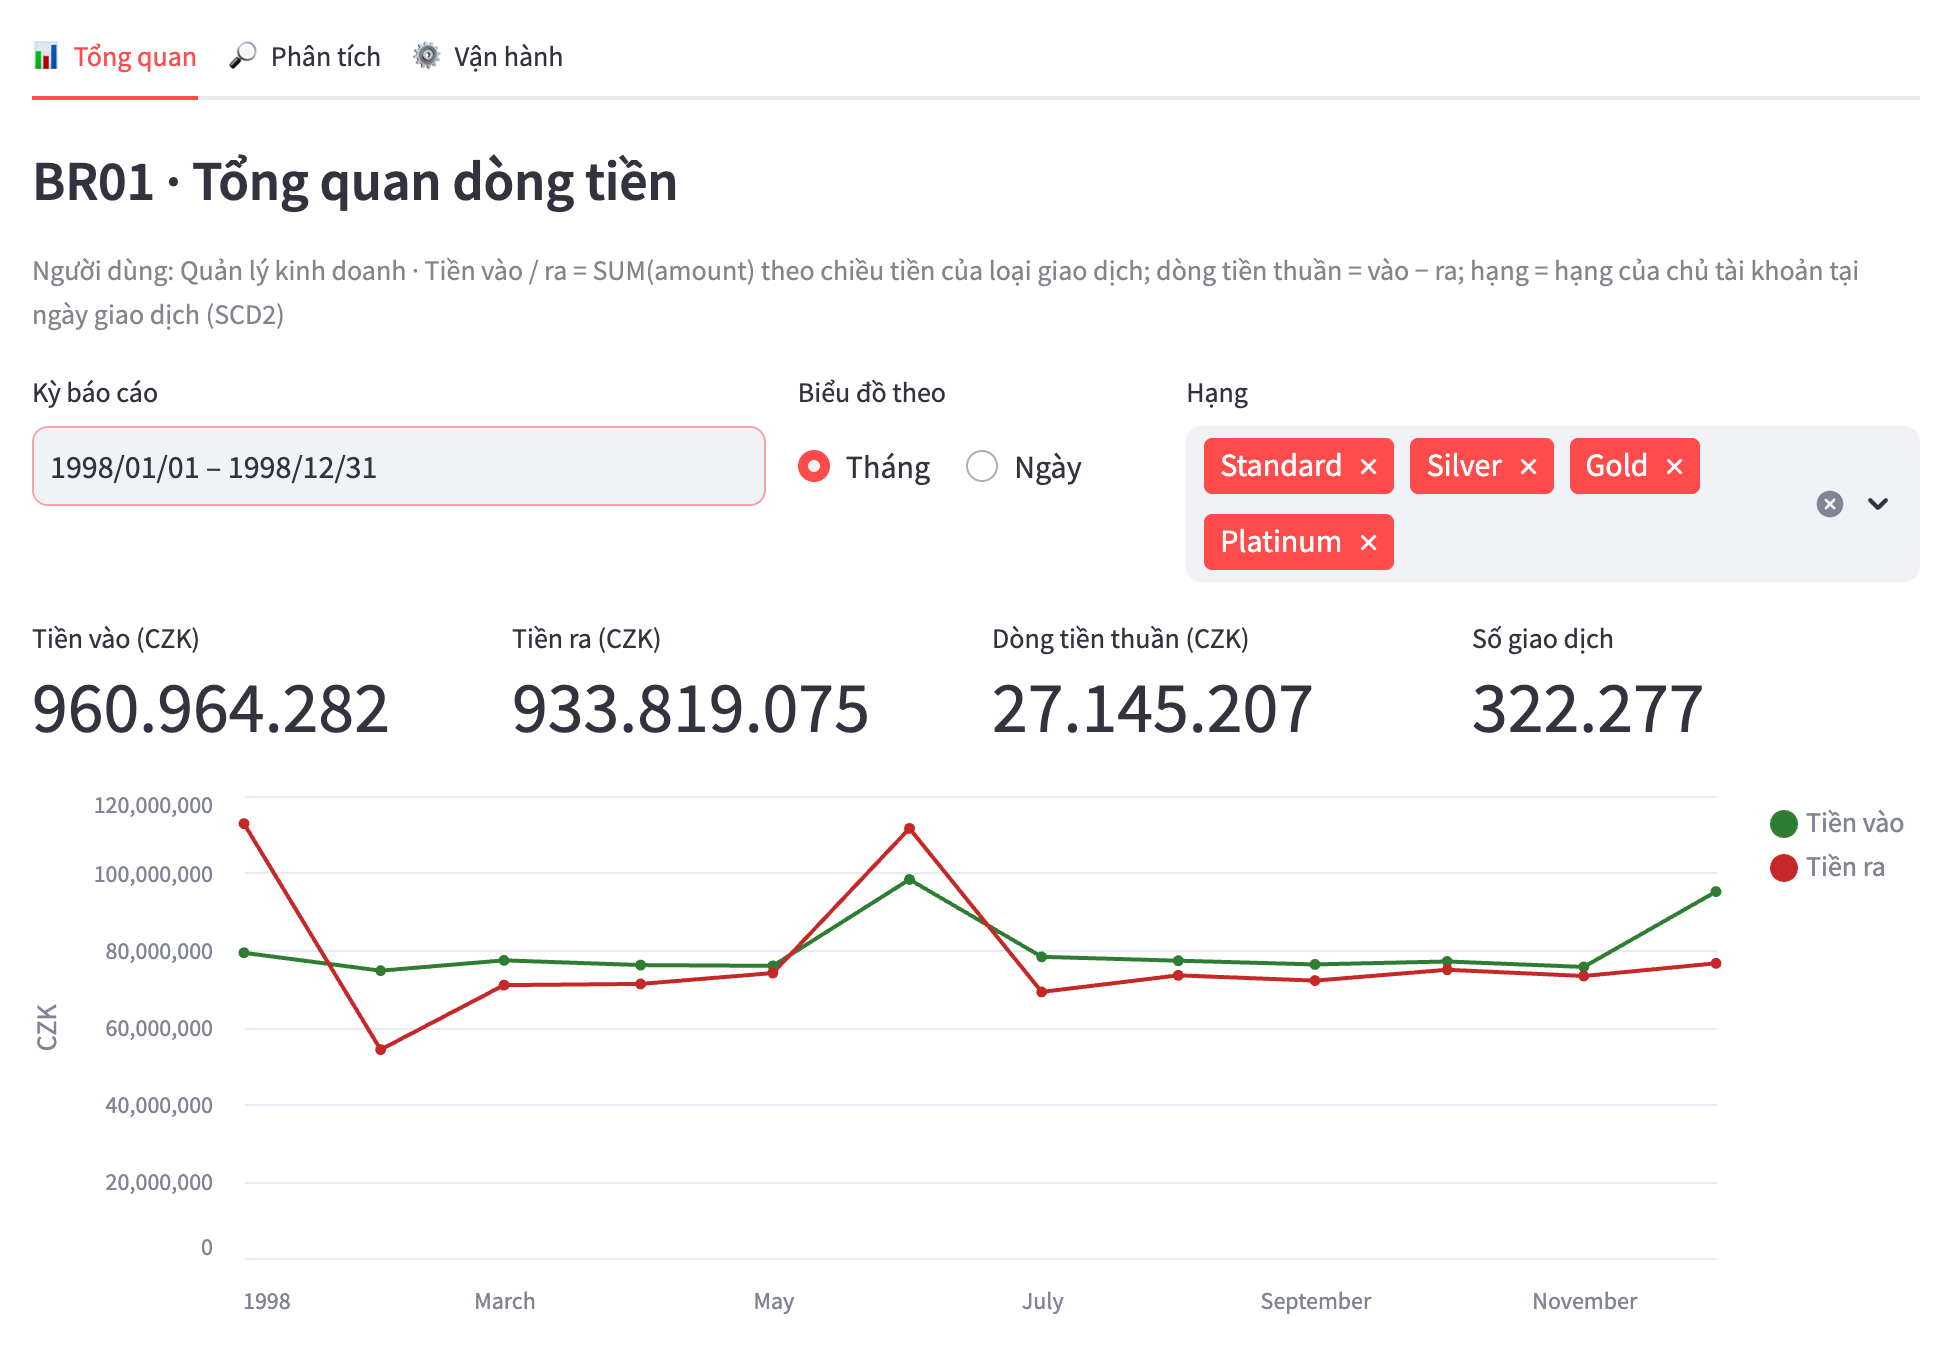
\includegraphics[height=0.78\textheight]{app_overview}\\
  \footnotesize Năm 1998: tiền vào 960.964.282 CZK, tiền ra 933.819.075 CZK, thuần 27.145.207 CZK, 322.277 giao dịch.
\end{frame}

\begin{frame}{Phân tích (U02, BR02): tra cứu tài khoản}
  \centering
  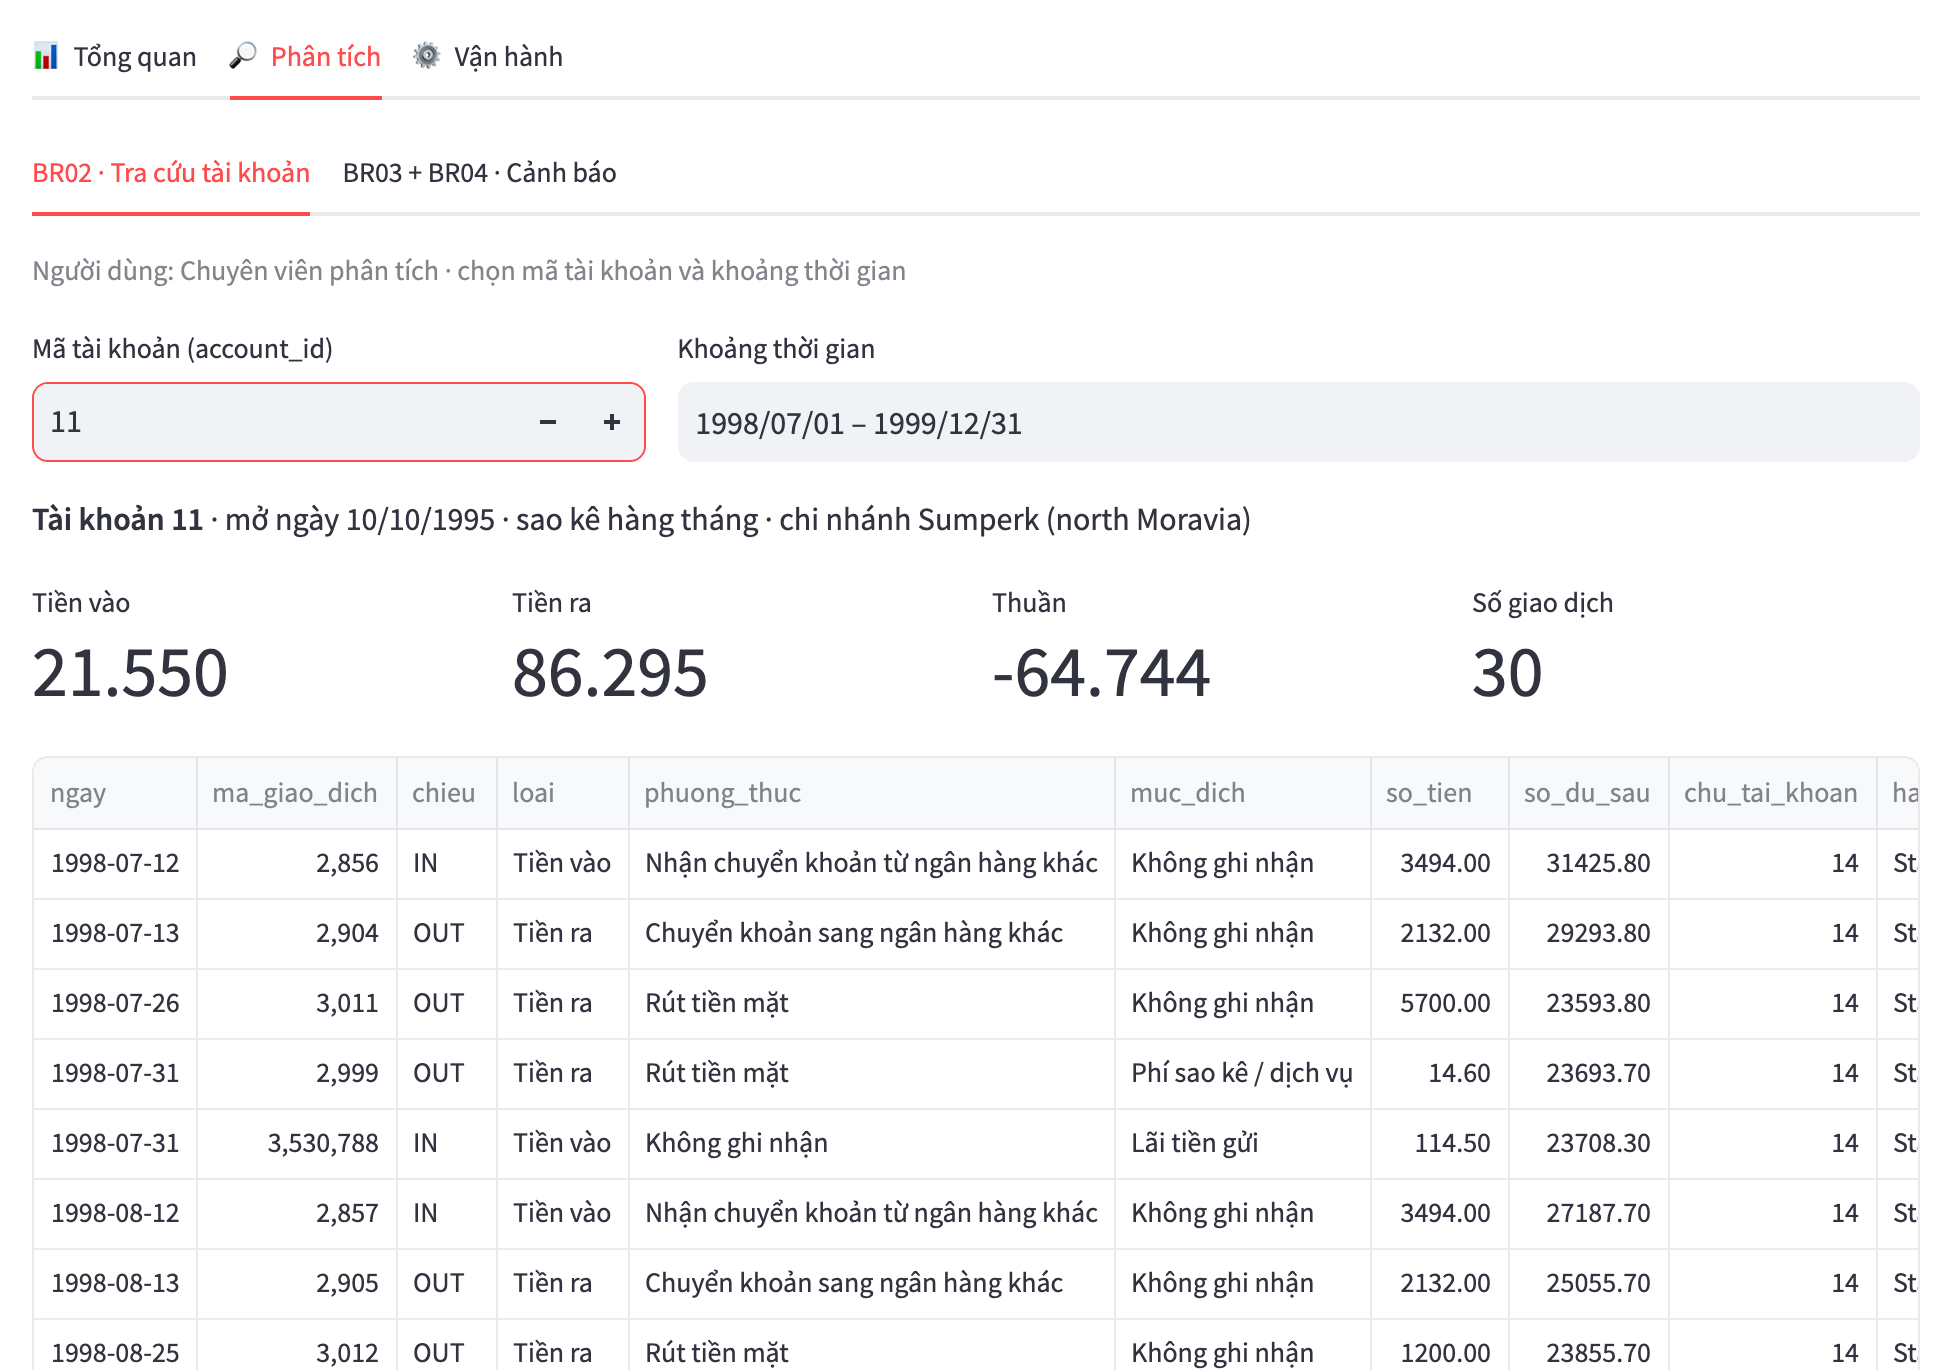
\includegraphics[height=0.78\textheight]{app_lookup}\\
  \footnotesize Tài khoản 11, 07/1998--12/1999: 30 giao dịch, gồm giao dịch rút 60.000 CZK của KB03.
\end{frame}

\begin{frame}{Phân tích (U02, BR03--BR04): cảnh báo}
  \centering
  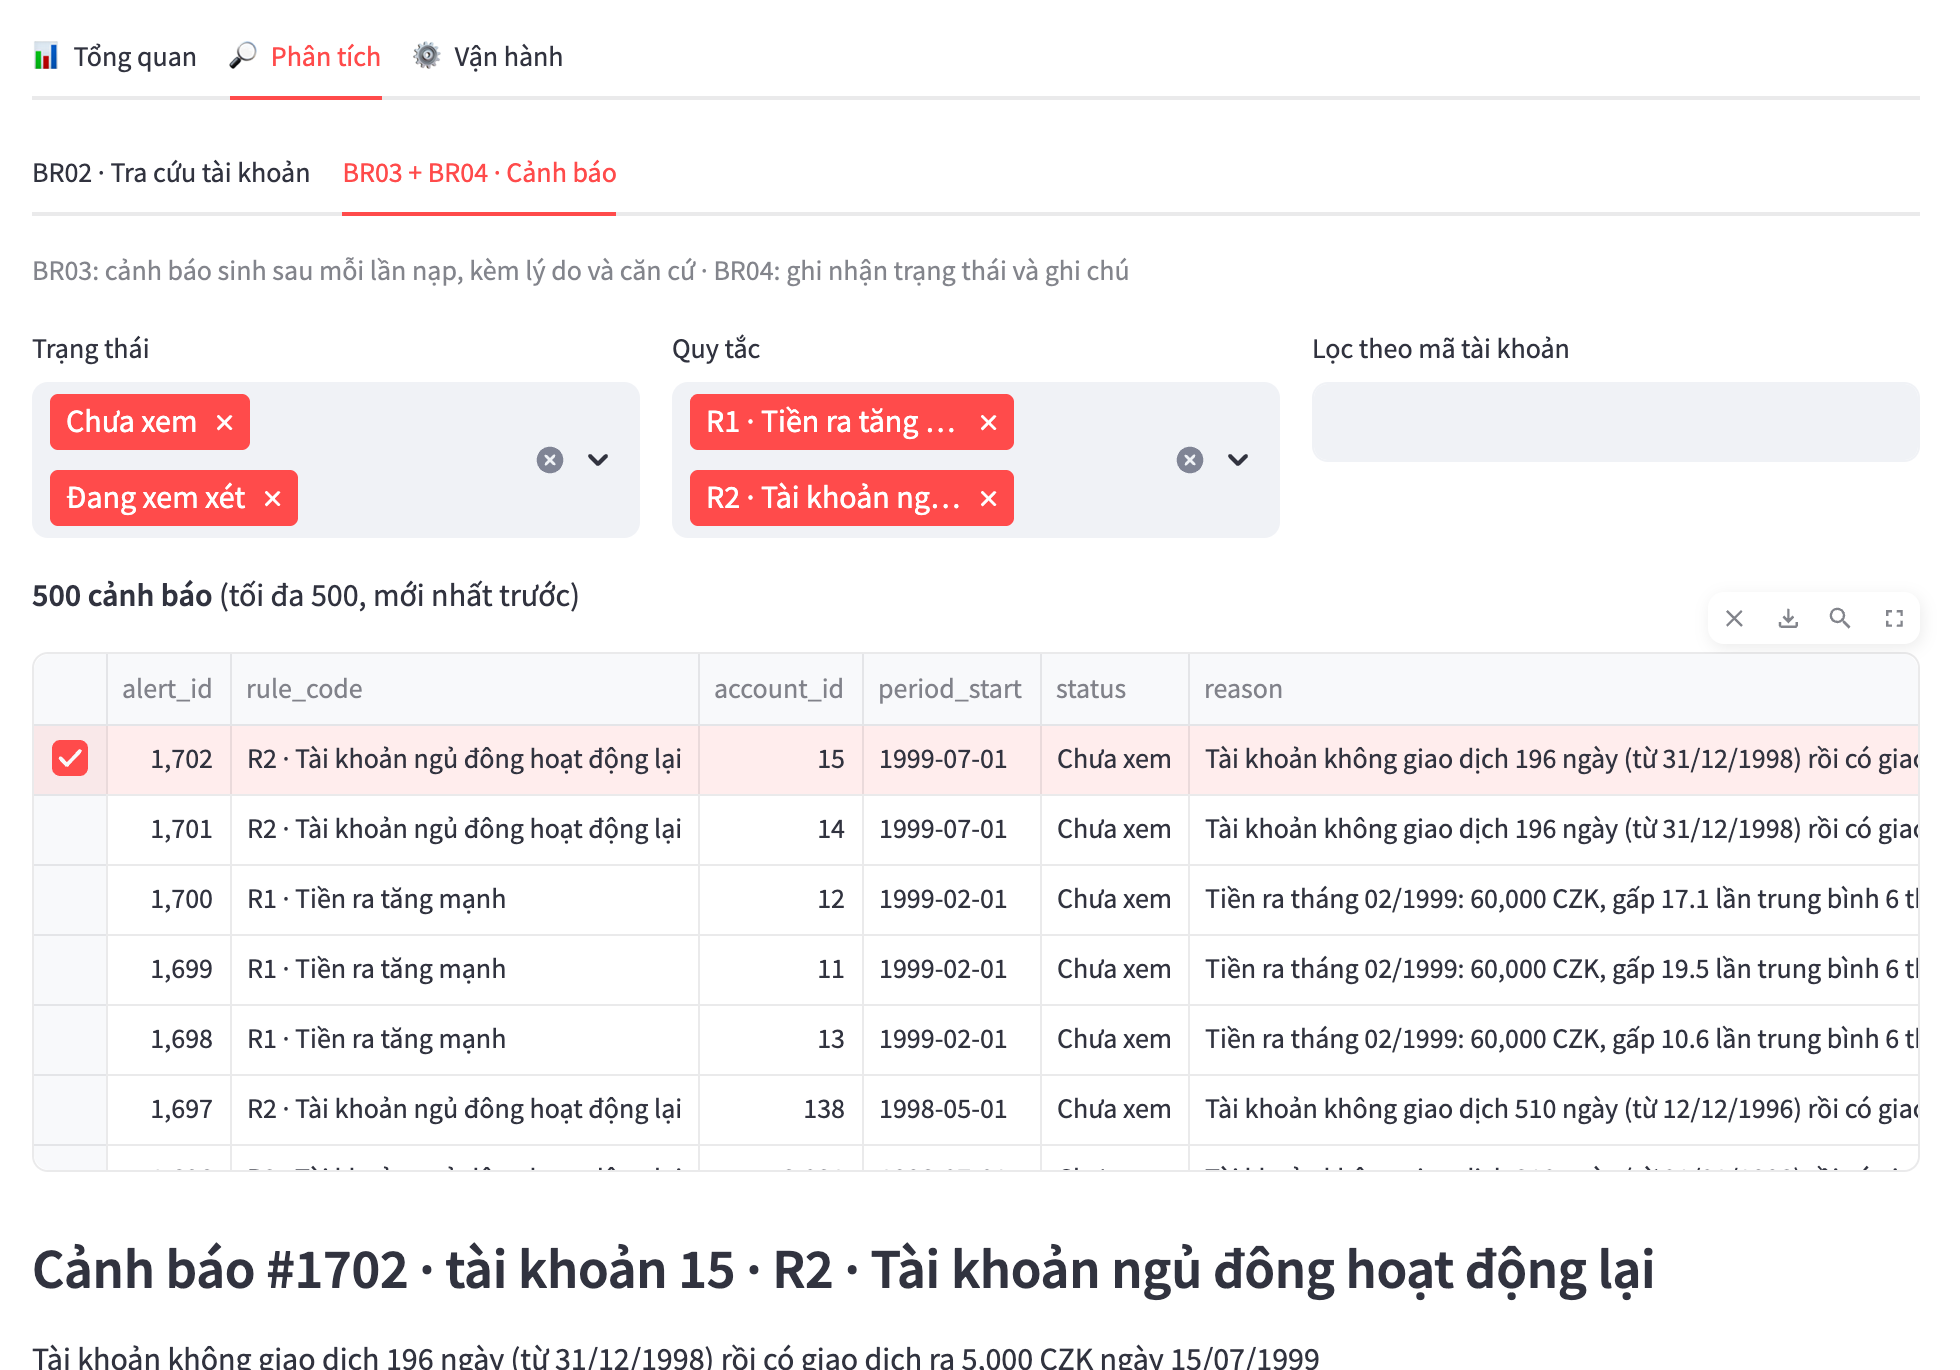
\includegraphics[height=0.78\textheight]{app_alert}\\
  \footnotesize Danh sách cảnh báo với quy tắc, tài khoản, kỳ, trạng thái, lý do; chọn một cảnh báo để xem căn cứ và xử lý.
\end{frame}

\begin{frame}{Vận hành (U03, BR08): lịch sử hạng thành viên}
  \centering
  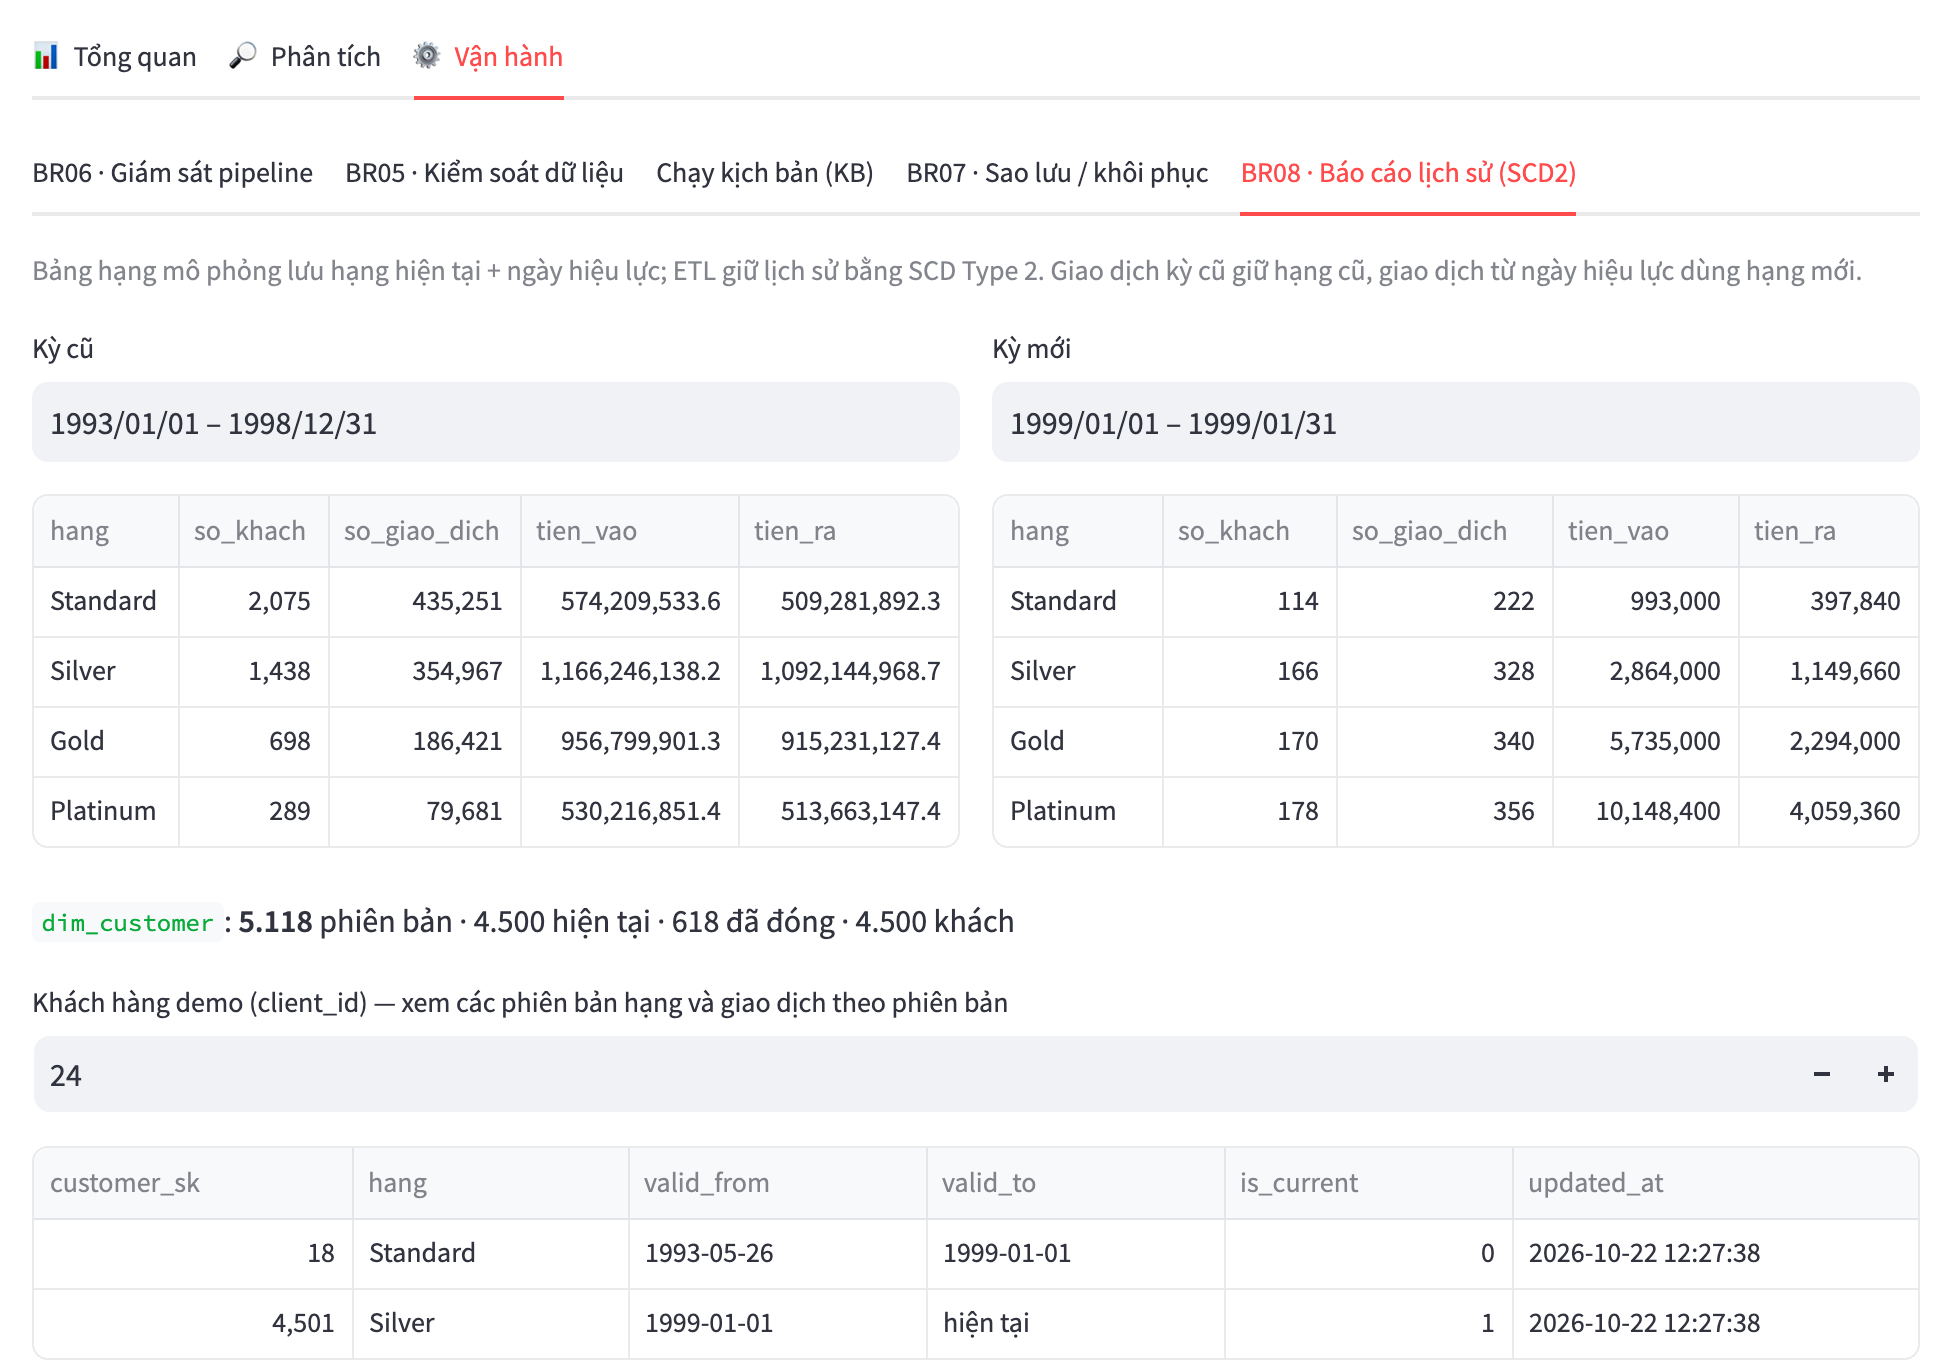
\includegraphics[height=0.78\textheight]{app_scd2}\\
  \footnotesize Báo cáo theo hạng kỳ cũ / kỳ mới; hai phiên bản hạng của khách 24.
\end{frame}

\begin{frame}{Vận hành (U03): chạy kịch bản}
  \centering
  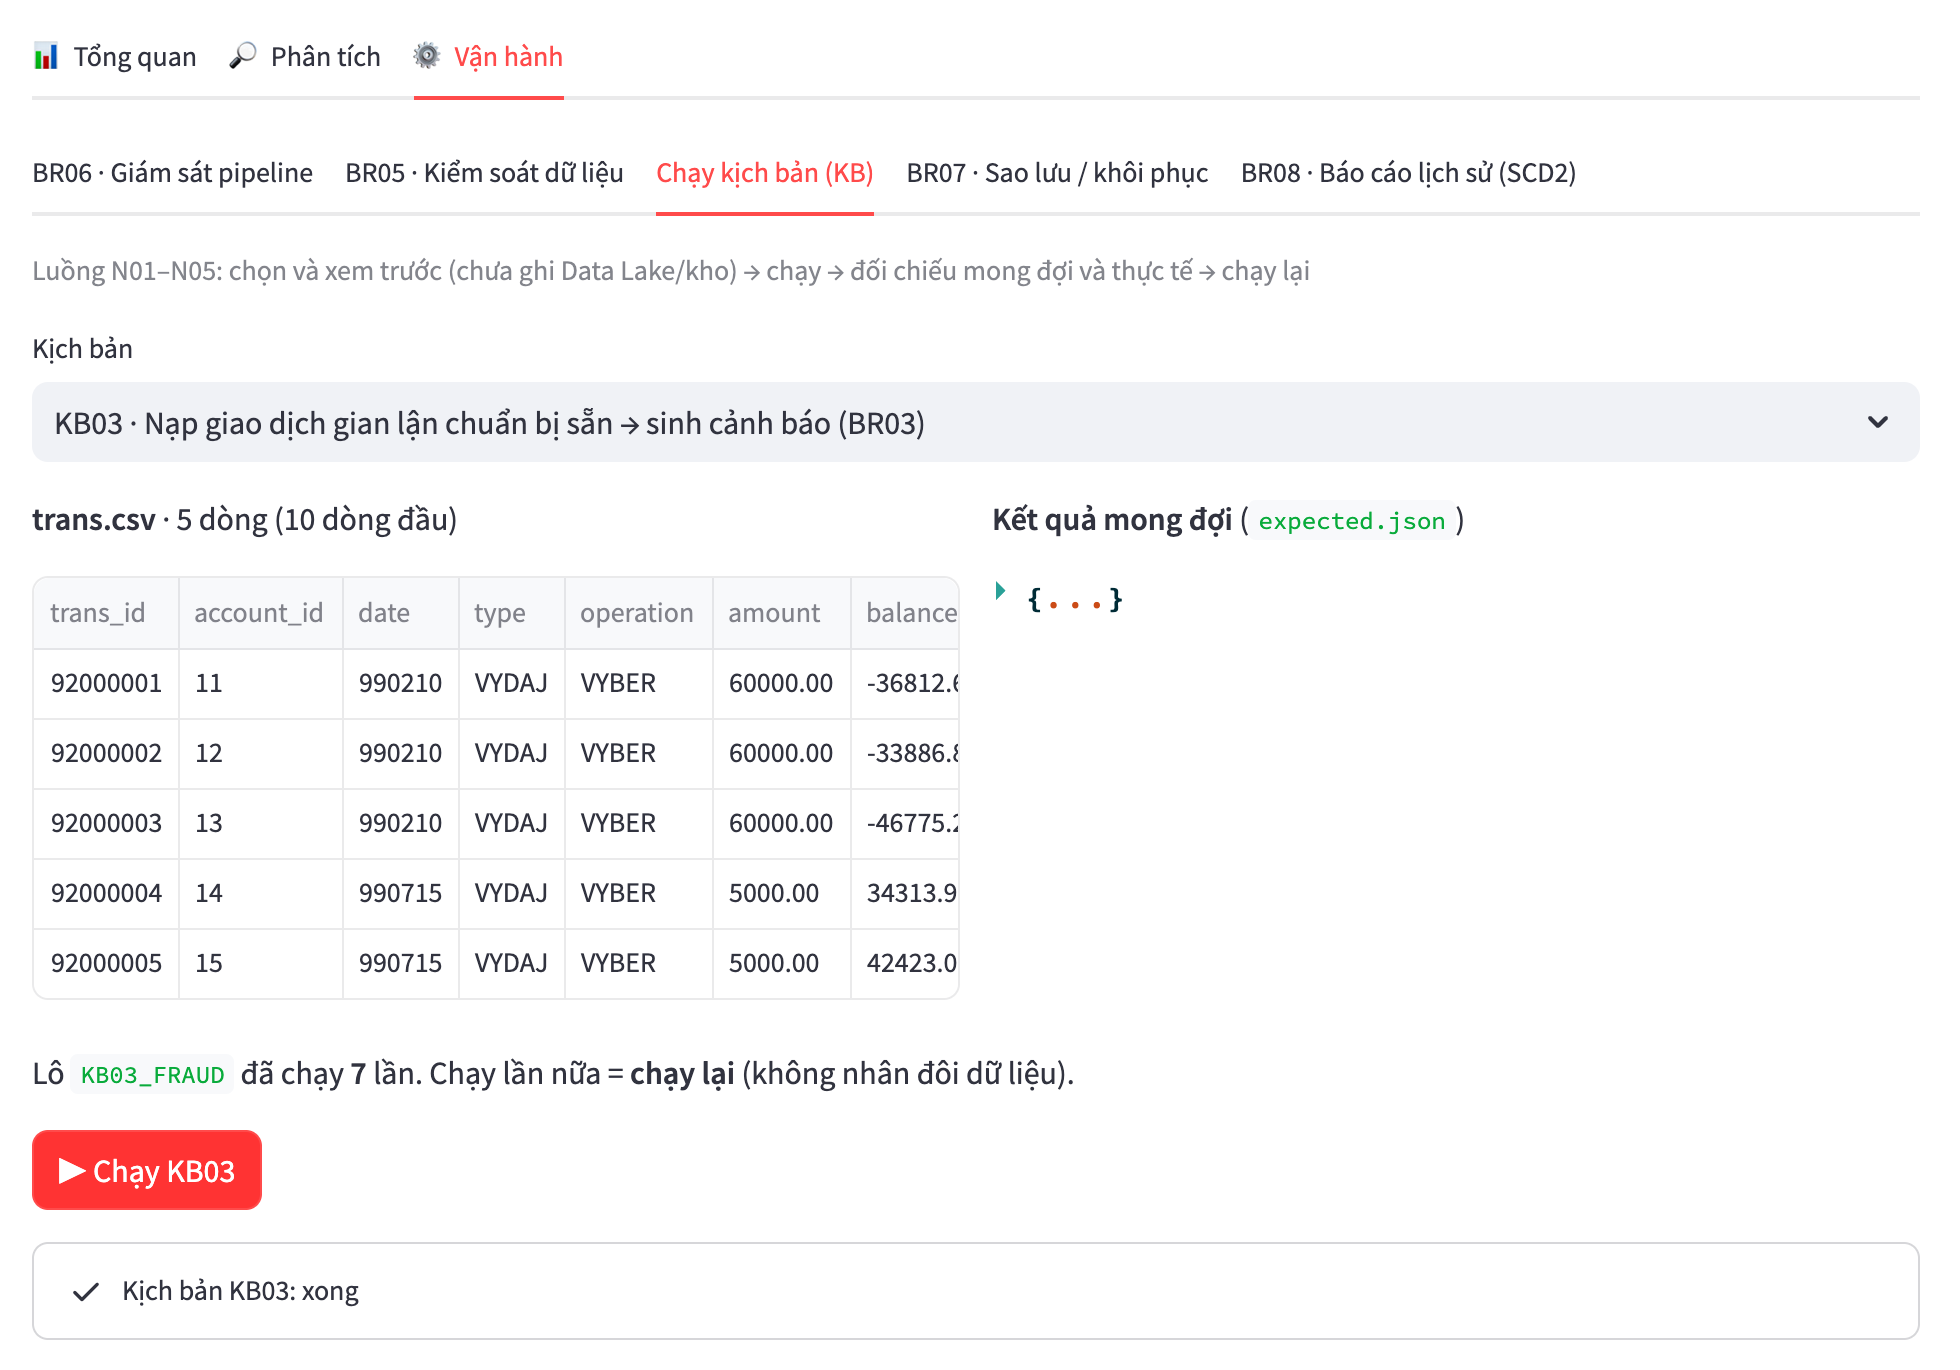
\includegraphics[height=0.78\textheight]{app_scenario_run}\\
  \footnotesize Xem trước đầu vào và kết quả mong đợi, rồi chạy lại KB03 (không nhân đôi dữ liệu).
\end{frame}

\begin{frame}{Trình tự demo trong video}
  \small
  \begin{enumerate}
    \item \textbf{KB01} Tổng quan: chọn năm 1998, đối chiếu tổng với truy vấn trên nguồn
    \item \textbf{KB05} Vận hành: chạy kịch bản dữ liệu lỗi → xem 10 bản ghi bị tách theo quy tắc
    \item \textbf{KB06} Vận hành: xem lần chạy, từng bước, lần chạy lỗi và nguyên nhân
    \item \textbf{KB03} chạy kịch bản gian lận → \textbf{KB02} tra cứu tài khoản 11 → xem cảnh báo và căn cứ
    \item \textbf{KB04} đổi trạng thái cảnh báo, ghi chú, xem lịch sử xử lý
    \item \textbf{KB08} xem báo cáo theo hạng kỳ cũ / kỳ mới, phiên bản của khách 24
    \item \textbf{KB07} sao lưu → nạp thêm → khôi phục → đối chiếu 5 nhóm số liệu
  \end{enumerate}
\end{frame}

%% =====================================================================
\section{Kết luận}

\begin{frame}{Kết luận và khuyến nghị}
  \begin{columns}[T]
    \column{0.55\textwidth}
    \small
    \begin{itemize}
      \item \textbf{Độ đúng:} 8/8 kịch bản, 38/38 kiểm tra; khớp nguồn tới từng xu; đổi hạng không làm thay đổi báo cáo cũ
      \item \textbf{Hiệu năng:} ClickHouse nhanh hơn 3--22 lần (7--28 lần ở ×10), gọn hơn 8,7 lần; kho vận hành PostgreSQL nhanh hơn 8--70 lần và tự chặn 5/5 loại lỗi
      \item \textbf{Hiệu quả khai thác:} 8/8 BR trên một ứng dụng, 1--3 thao tác, trả lời dưới 0,5 giây
    \end{itemize}
    \column{0.42\textwidth}
    \begin{block}{Khuyến nghị}
      \small Kho dữ liệu dùng \textbf{lưu theo cột} (người dùng chủ yếu tổng hợp); dữ liệu vận hành dùng \textbf{cơ sở dữ liệu quan hệ} (sửa tại chỗ, ràng buộc).\\[4pt]
      Truy vấn tra cứu nên lọc bảng fact theo khóa của chính nó trước.
    \end{block}
  \end{columns}
\end{frame}

\begin{frame}{Hạn chế và hướng phát triển}
  \begin{columns}[T]
    \column{0.48\textwidth}
    \textbf{Hạn chế}
    \small
    \begin{itemize}
      \item Dữ liệu đến năm 1998, khoảng 1 triệu giao dịch; ×10 là dữ liệu nhân bản
      \item Hạng thành viên và kịch bản là mô phỏng
      \item Chưa có số dư cuối kỳ, chuyển tiền nội bộ
      \item Ứng dụng chưa phân quyền; kho vận hành ngoài phạm vi sao lưu
    \end{itemize}
    \column{0.48\textwidth}
    \textbf{Hướng phát triển}
    \small
    \begin{itemize}
      \item Phân quyền theo nhóm người dùng
      \item Thêm quy trình nghiệp vụ: khoản vay, lệnh chuyển tiền định kỳ
      \item Đo ở ×50 và trên cluster
      \item Phát hiện bất thường bằng mô hình học, đánh giá trên cùng các kịch bản
    \end{itemize}
  \end{columns}
\end{frame}

\begin{frame}[plain]
  \centering
  \vfill
  {\color{navy}\Huge\bfseries Cảm ơn thầy cô và các bạn}\par\bigskip
  {\Large Hỏi và đáp}\par\vfill
  \footnotesize Mã nguồn: \url{https://github.com/quanndc/data-engineer-bank-project}
\end{frame}

\end{document}
